\title{LEZIONE 7 16/04/2020}\newline
\textbf{link} \href{https://web.microsoftstream.com/video/16847746-6bdf-4d6b-bcbb-e5829a862801}{clicca qui}
\section{Statica dei sistemi di corpi rigidi}
\subsection{Equazioni cardinali della statica dei sistemi di corpi rigidi}
Come fra punto materiale e corpo rigido, anche fra corpo rigido e sistema di copri rigido, le equazioni cardinali del corpo rigido non sono più una condizione sufficiente per l'equilibrio del sistema.\newline
\newline
Perchè il sistema di copri rigidi sia in equilibrio bisogna che sia in equilibrio ogni parte del sistema stesso sotto l'azione delle forze esterne che competono su ciascun copro e sotto le azioni delle forze che traducono le azioni delle parti contigue. In altre parole affinchè il sistmea di corpi rigidi sia in equilibrio bisogna che lo sia ogni sua parte sotto le forze esterne e interne, e attive e reattive. \newline
\newline
Vediamo le \textbf{equazioni cardinali della statica dei sistemi di corpi rigidi}:
\[
    \begin{cases}
        \sum_{j} \vec{F}_{j,i} = 0\\
        \sum_{j} (P_{j,i} - 0) \land \vec{F}_{j,i} + \sum_{k} \vec{C}_{k,i} = 0
    \end{cases}
\]
per $i = 1,2,\dots, n_c$.\newline
\newline
Le forze \textbf{attive} sono tutte le forze \textbf{esterne} che possono essere applicate al sistema, le forze \textbf{reattive} sono invece le forze vincolari, le forze \textbf{interne} sono le forze che traducono gli effetti dei copri contigui a quello considerato.\newline
\newline
Nella risoluzioni di problemi di statica di sistemi di corpi rigidi solitamente si procede isolando uno ad uno tutti i corpi che li costituiscono singolarmente, analizzando tutte le forze in gioco. In seguito si impostano le $3 \cdot n_c$ equazioni cardinali in modo da poter risolvere al più $3 \cdot n_c$ incognite.\newline
\newline
In particolare le equazioni cardinali ci permettodo di:
\begin{itemize}
    \item calcolare le reazioni vincolari incognite;
    \item se sono note le forze esterne, di calcolare la posizione di equilibrio incognita;
    \item oppure, se è nota la posizione di equilibrio, ci permettono di calcolare le forze esterne che ci permettono di mantenere tale posizion.
\end{itemize}
Questi tre punti valgono se e solo se il sistema è isostatico oppure ipostatico, cioè se $n_v \leq 3 \cdot n_c$.\newline
\newline
\textbf{es.} \newline
[immagine dagli appunti del prof]
\begin{center}
    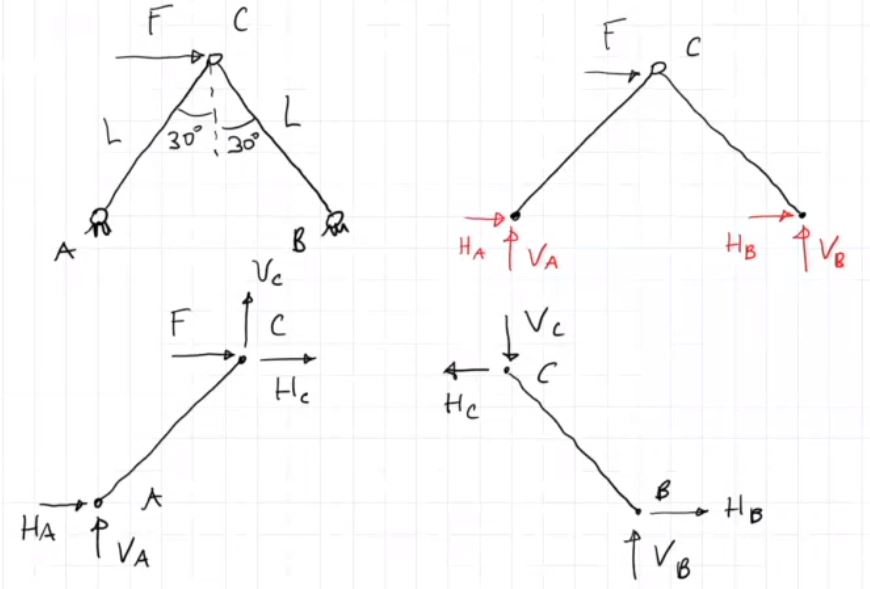
\includegraphics[height=5cm]{../lezione7/img1.JPG}
\end{center}
Le incognite sono solo le reazioni vincolari $H_A, V_A, H_B, V_B, V_C, H_B$, che sono $6$, ma siccome abbiamo due corpi abbiamo $3 \cdot n_c = 6$ equazioni.\newline
\newline
Ora bisognerebbe solo impostare le equazioni cardinali e risolvere, ma vediamo un metodo più furbo per risolvere l'esercizio.\newline
E' sufficiente accorgersi di conoscere la direzione delle reazioni vincolari sia in $A$, sia in $B$:\newline
[immagine dagli appunti del prof]
\begin{center}
    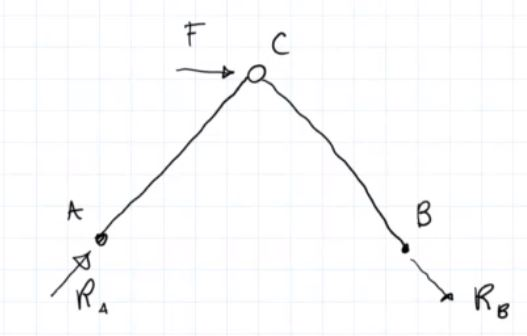
\includegraphics[height=3cm]{../lezione7/img2.JPG}
\end{center}
Vediamo per esempio l'asta $AC$:\newline
[immagine dagli appunti del prof]
\begin{center}
    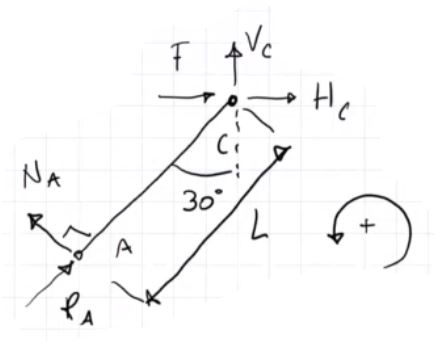
\includegraphics[height=3cm]{../lezione7/img3.JPG}
\end{center}
Notiamo che nell'analisi dei momenti rispetto al polo $C$, l'unica forza che non ha braccio nullo è $N_A$, tutte le altre hanno retta di applicazione passante per il punto $C$ (e quindi braccio nullo), quindi 
\[
    M_C = 0 \rightarrow -N_A L = 0
\]
dove il segno negativo viene dal fatto che si prende per convenzione una rotazione antioraria positiva e che la forza $N_A$ fa ruotare l'asta attorno al polo in senso orario.\newline
Lo stesso discorso si applica anche all'asta $CB$.\newline
\newline
Perchè la reazione vincolare abbia la stessa direzione dell'asta che staimo considerando, devono verificarsi due condizioni:
\begin{itemize}
    \item ci siano due cerniere agli estremi;
    \item non si abbiamo forze o momenti concetrati sull'asta se non negli estremi.
\end{itemize}
Quando queste condizioni sono rispettate, si dice che l'asta è una \textbf{biella}, cioè la reazione vincolare è diretta parallelamente all'asta.\newline
\newline
Risolviamo ora questo esercizio sfruttando questo concetto:\newline
[immagine dagli appunti del prof]
\begin{center}
    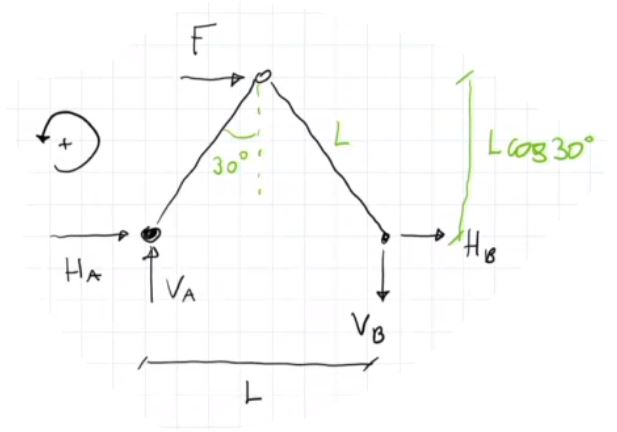
\includegraphics[height=3cm]{../lezione7/img4.JPG}
\end{center}
\[
    M_A = 0 \rightarrow -FL cos(30^0) - V_B L = 0 \rightarrow V_B = -F cos(30^0) = - \frac{\sqrt{3}}{2}F
\]
Sapendo che l'asta $CB$ è una biella e che la sua reazione vincolare ha direzione parallela all'asta posso scrivere:
\[
    R_B = \frac{V_B}{cos(30^0)} = -F
\]
Per cui la sola componente orizzonatale diventa 
\[
    H_B = \frac{F}{2}
\]
da cui, uguagliando le forze lungo l'asse delle $X$, ottengo:
\[
    R_x = 0 \rightarrow  H_A + F - H_B = 0 \rightarrow H_A = -\frac{F}{2}
\]
uguagliando sull'asse delle $Y$, invece, ottengo:
\[
    R_y = 0 \rightarrow  V_A + V_B = 0 \rightarrow V_A = - V_B = - \frac{\sqrt{3}}{2}
\]
[immagini dagli appunti del prof]
\begin{center}
    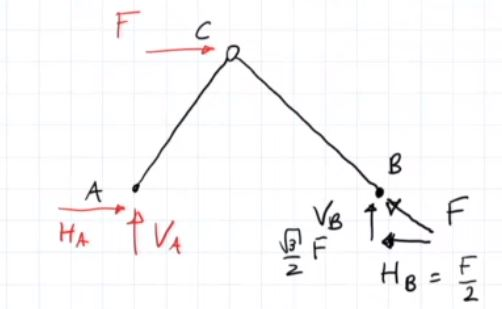
\includegraphics[height=3cm]{../lezione7/img5.JPG}
\end{center}
\begin{center}
    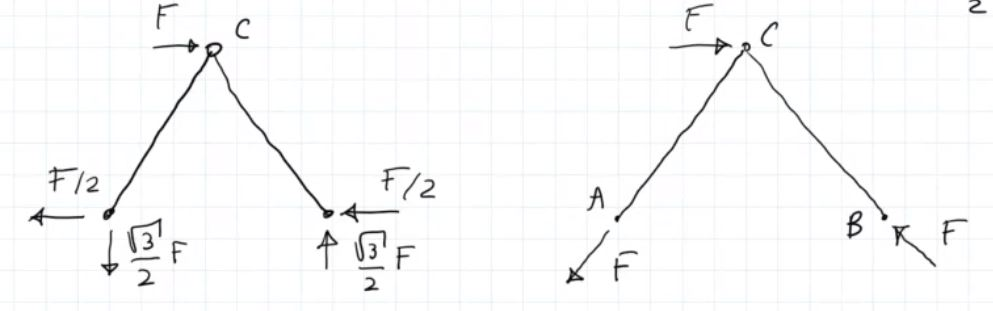
\includegraphics[height=3cm]{../lezione7/img6.JPG}
\end{center}
\rule{\textwidth}{0,4pt}
\subsection{Azioni interne}
Uno dei problemi della meccanica è quello di indagare lo stato di sollecitamentento di un componente all'interno di un sistema, ovvero capire quali sono le sezioni del corpo maggiormente sollecitate dalle forze esterne al sistema.\newline
\newline
In questo corso studieremo gli stati di sollecitamento di una certa sezione di \textbf{travi snelle} in equilibrio.\newline
\newline
[immagine dagli appunti del prof]
\begin{center}
    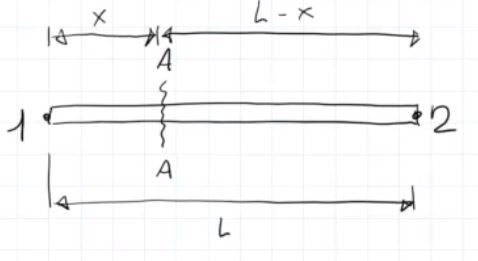
\includegraphics[height=3cm]{../lezione7/img7.JPG}
\end{center}
Per studiare lo stato di sollecitamento della tave in figura nella sezione $A$ possiamo suddividere la trave in due sotto travi con un \textbf{incastro fittizio} e quindi isolarle e studiarne le forze vincolari:\newline
[immagine dagli appunti del prof]
\begin{center}
    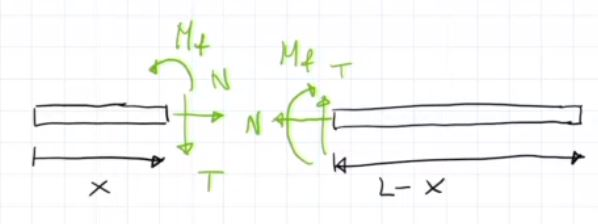
\includegraphics[height=3cm]{../lezione7/img8.JPG}
\end{center}
dove $M_f$ prende il nome di \textbf{momento flettente}, $N$ prende il nome di \textbf{azione assiale}, $T$ prende il nome di \textbf{azione di taglio}. Queste tre assieme costituiscono le \textbf{azioni interne}.\newline
\newline
Per convenzione l'azione assiale $N$ è positiva se mette in trazione la sezione considerata, l'azione di taglio è positiva se fa ruotare in senso antiorario la sezione ocnsiderata e il momento flettente è positiva se va atendere le fibbre della parte inferiore dell'elemento considerato.\newline
\newline
\textbf{es.} Riprendiamo un esempio della lezione scorsa di cui avevamo già valutato le forze:\newline
[immagine dagli appunti del prof]
\begin{center}
    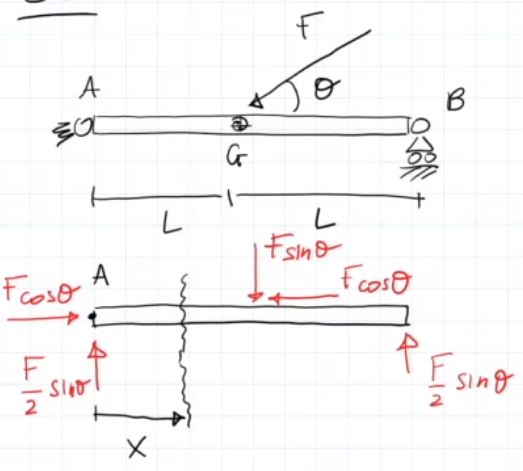
\includegraphics[height=3cm]{../lezione7/img9.JPG}
\end{center}
Volendo studiare le azioni interne al variare di $x$ lungo la trave, troviamo in due diversi casi poichè nel punto $G$ sono presenti delle forze applicate:
\begin{itemize}
    \item $0\leq x < L$
    \item $L\leq x \leq 2L$
\end{itemize}
\ \newline
Per il caso $0\leq x < L$:\newline
[immagine dagli appunti del prof]
\begin{center}
    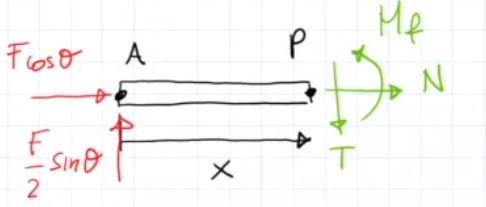
\includegraphics[height=3cm]{../lezione7/img10.JPG}
\end{center}
Applichiamo le equazioni cardinali della statica usando il polo $P$ per i momenti:
\[
    \begin{cases}
        F cos(\theta) + N = 0\\
        \frac{F}{2} sin(\theta) - T = 0\\
        - \frac{F}{2} sin(\theta) x + M_f = 0
    \end{cases} \rightarrow  \begin{cases}
        N = - F cos(\theta)\\
        T = \frac{F}{2} sin(\theta)\\
        M_f = \frac{F}{2} sin(\theta) x
    \end{cases}
\]
\ \newline
Per il caso $L\leq x \leq 2L$:
[immagine dagli appunti del prof]
\begin{center}
    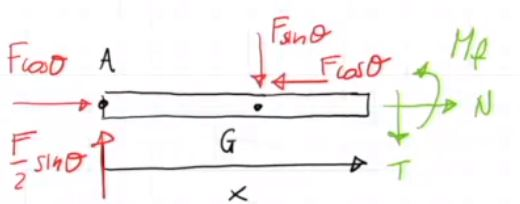
\includegraphics[height=3cm]{../lezione7/img11.JPG}
\end{center}
Applichiamo le equazion icardinali della statica:
\[
    \begin{cases}
        F cos(\theta) - F cos(\theta) + N = 0\\
        \frac{F}{2} sin(\theta) - F sin(\theta) - T = 0\\
        - \frac{F}{2} sin(\theta) x + F sin(\theta) (x-L) + M_f = 0
    \end{cases} \rightarrow  \begin{cases}
        N = 0\\
        T = - \frac{F}{2} sin(\theta)\\
        M_f = F L sin(\theta) - \frac{F x}{2} sin(\theta)
    \end{cases}
\]
\ \newline
Unendo i due risultati posso scrivere un diagramma che mi mostra le tre azioni interne in dipendenza del valore di $x$:\newline
[immagine dagli appunti del prof]
\begin{center}
    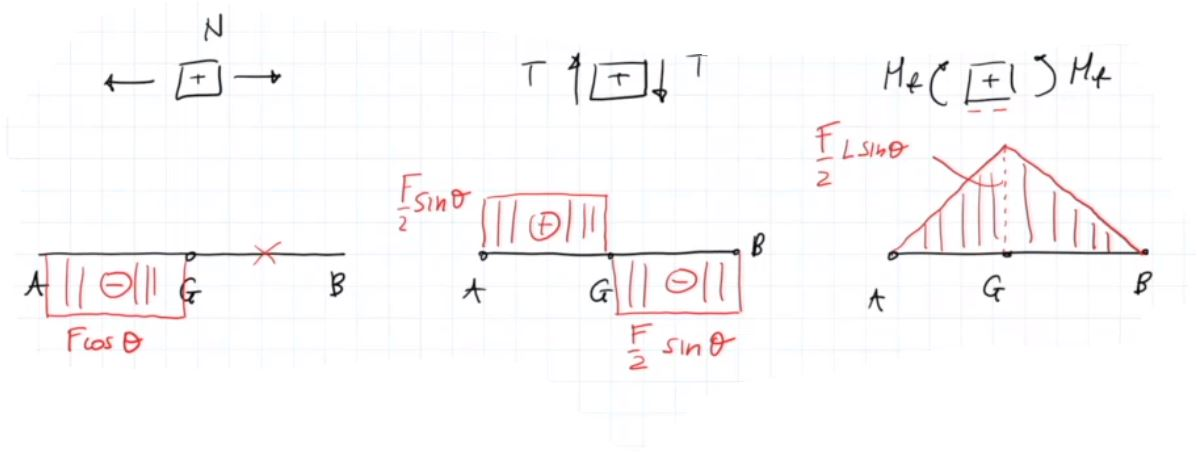
\includegraphics[height=4cm]{../lezione7/img12.JPG}
\end{center}
\ \newline
La \textbf{prima verifica} che bisgna fare per capire se i risultati ottenuti sono sensati è che agli estremi (sui vincoli) i valori delle reazioni vincolari agli estremi coincidano con i valori delle azioni interne. In questo esempio per i vincoli in $A$ le azioni assiali devono coincidere con $H_A$ e le azioni di taglio devono coincidere con $V_A$, nel punto $B$ invece abbiamo solo le azioni di taglio e devono coincidere con $V_B$.\newline
\newline
Come \textbf{secondo verifica} si possono cercare i punti in cui ci sono delle discontinuità nelle azioni interne (si vede bene nel diagramma riportato poco fa - ultima immagine). Questi punti o discontinuità possono esistere solo se sono presenti delle forze o dei momenti concentrati. Inoltre la discontinuità dovrà essere uguale al valore della forza che sto applicando. Nel nostro esempio la discontinuità in $G$ dell'azione assiale dovrà essere pari a $F cos(\theta)$, mentre la discontinuità dell'azione di taglio dovrà essere pari a $F sin(\theta)$.\newline
\rule{\textwidth}{0,4pt}